\documentclass[journal,twocolumn,10pt, a4paper]{article}                                
\usepackage[top=0.95in, bottom=1in, left=0.95in, right=0.95in]{geometry}
\usepackage{array}
\usepackage[colorlinks,linkcolor={black},citecolor={blue!80!black},urlcolor={blue!80!black}]{hyperref}
\usepackage[parfill]{parskip}
\usepackage{lmodern}
\renewcommand*\familydefault{\sfdefault}
\setlength{\columnsep}{40pt}
\usepackage{watermark}

\usepackage{circuitikz}
\usetikzlibrary{circuits.logic.IEC,calc}
\usepackage{tikz}
\usepackage{amsmath}
\usepackage{setspace}
\usetikzlibrary{shapes, arrows, chains, decorations.markings,intersections,calc}
\usepackage{lipsum}
\usepackage{xcolor}
\usepackage{listings}
\usepackage{float}
\usepackage{titlesec}
\usepackage{amsmath}
\usepackage{tabularx}
\usepackage{algorithm2e}
\usepackage{./karnaugh-map}
\usepackage[utf8]{inputenc}
\usepackage{pgfplots}
\usepackage{listings}
\usepackage{placeins}
\usepackage{graphicx}


\begin{document}


\lstset{                                   
language=C++,                             
basicstyle=\ttfamily\footnotesize,         
breaklines=true,                           
frame=lines}


\title{ASSEMBLY ASSIGNMENT}
\author{Tanyala Srihitha\\srihithatanyala@gmail.com}
\maketitle
\tableofcontents
 
\section{Problem}

(GATE EC-2020)\\

Q.No 50. For the components in the sequential circuitshown below,tpd is the propagation delay, tsetup is the setup time, and thold is the hold time. the maximum clock frequency(rounded off to the nearest integer),at which the given circuit can operate reliably, is        MHz.
\\


\begin{figure}[!h]
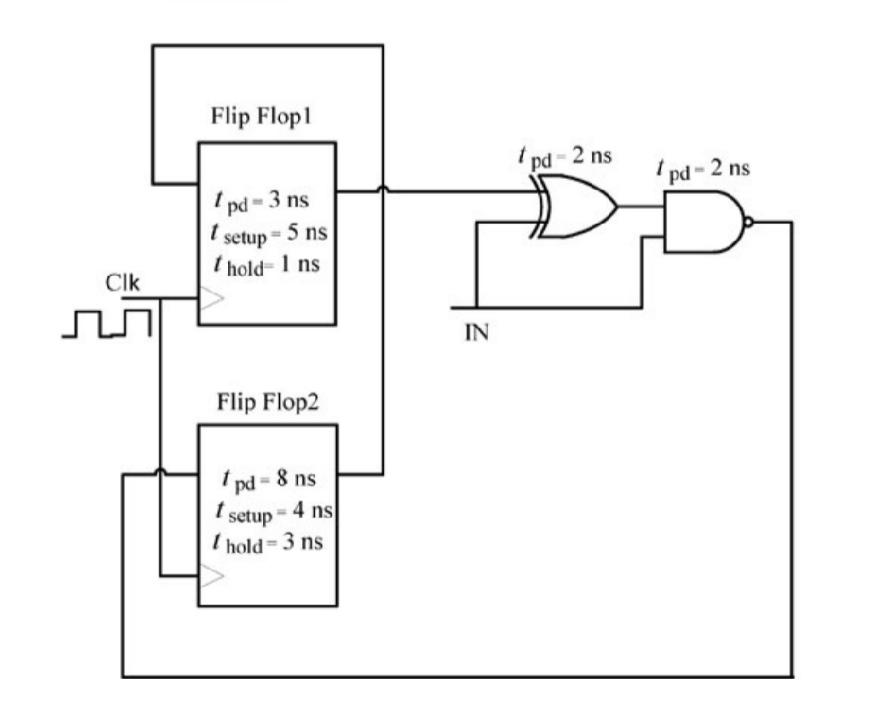
\includegraphics[width=\columnwidth]{./figs/ff.jpg}
\caption{}
\label{fig:Figure 1}
\end{figure}

\section{Components}
The components required are given in Table \ref{tab:Components}                    
\begin{table}[!h]
\centering
\begin{center}
\begin{tabularx}{0.45\textwidth}{|>{\centering\arraybackslash}X|>{\centering\arraybackslash}X|>{\centering\arraybackslash}X|}
\hline
\textbf{Component} & \textbf{Value} & \textbf{Quantity}\\
\hline
Arduino UNO & - & 1\\                    
\hline
Breadboard & - & 1\\
\hline                                   
7447 IC & - & 1\\
\hline
Seven segment display & - & 1\\
\hline
Resistor & 200ohms & 1\\                
\hline                                   
Jumper wires & M-M & 20\\               
\hline
\end{tabularx}
\end{center}


\caption{}
\label{tab:Components}                     
\end{table}


\subsection{Arduino}
The Arduino Uno has some ground pins, analoginput pins A0-A3 and digital pins D1-D13 that can be used for both input as well as output. It also has two power pins that can generate 3.3V and 5V.
\subsection{Seven Segment Display}
The seven segment display has eight pins, a,b, c, d, e, f, g and dot that take an active LOW input, i.e. the LED will glow only if the input is connected to ground. Each of these pins is connected to an LED segment. The dot pin is reserved for the · LED.

\section{Implementation}

\subsection{Truth Table}
From the above equation, truth table is given in Table \ref{tab:Truth Table}
\begin{table}[!h]
\centering
\begin{center}                                   \begin{tabularx}{0.35\textwidth}{|>{\centering\arraybackslash}X|>{\centering\arraybackslash}X|>{\centering\arraybackslash}X|>{\centering\arraybackslash}X|}                                        
\hline                                          
\textbf{IN}&\textbf{Q1}&\textbf{Q2}&\textbf{Qy}\\
\hline                                           
0 & 0 & 0 & 1 \\                                 
\hline                                           
0 & 0 & 1 & - \\                                 
\hline
0 & 1 & 0 & - \\                          
\hline                                      
0 & 1 & 1 & 1 \\
\hline                                         
1 & 0 & 0 & 0 \\                  
\hline                     
1 & 0 & 1 & - \\           
\hline                 
1 & 1 & 0 & - \\
\hline
1 & 1 & 1 & 1 \\
\hline                                      
\end{tabularx}
\end{center}

\caption{}
\label{tab:Truth Table}
\end{table}\\


\subsection{K-map}
From the above truth table, Fig \ref{fig:Fig 2} represents the K-map:
\begin{figure}[!h]
\documentclass{article}
\usepackage[top=0.95in, bottom=1in, left=0.95in, right=0.95in]{geometry}
\usepackage{array}
\usepackage[colorlinks,linkcolor={black},citecolor={blue!80!black},urlcolor={blue!80!black}]{hyperref}
\usepackage[parfill]{parskip}
%% Arial-like font
\usepackage{lmodern}
\renewcommand*\familydefault{\sfdefault}
\setlength{\columnsep}{40pt}
%Napier logo top right
\usepackage{watermark}
%Lorem Ipusm dolor please don't leave any in you final report ;)
\usepackage{circuitikz}
\usetikzlibrary{circuits.logic.IEC,calc}
\usepackage{tikz}
\usepackage{amsmath}
\usepackage{setspace}
\usetikzlibrary{shapes, arrows, chains, decorations.markings,intersections,calc}
\usepackage{lipsum}
\usepackage{xcolor}
\usepackage{listings}
%give us the Capital H that we all know and love
\usepackage{float}
%tone down the line spacing after section titles
\usepackage{titlesec}
%Cool maths printing
\usepackage{amsmath}
\usepackage{tabularx}
%PseudoCode
\usepackage{algorithm2e}
\usepackage{karnaugh-map}
\usepackage[utf8]{inputenc}
\usepackage{pgfplots}
\begin{document}
\begin{karnaugh-map}[4][2][1][$QR$][$P$]
        \maxterms{0,2,3,4}                                  \minterms{1,5,6,7}                                                                                      \implicant{1}{5}
        \implicant{7}{6}
\end{karnaugh-map}
\end{document}

\caption{}
\label{fig:Fig 2}
\end{figure}

\subsection{Boolean Expression}
By Solving the above K-map, we get a boolean equation as: $Qy=Q1Q2+{Q1^\prime}{Q2^\prime}{In^\prime}$\\
$Qy=Q1Q2+{In^\prime}$


\section{Hardware}
\begin{enumerate}
\item Connect the arduino to computer and upload the code in to the arduino.
\item Make 2,3,4 as input pins and 8,9,10 as output pins.
\item By changing inputs check the corresponding outputs.
\end{enumerate}

\section{Software}
\lstinputlisting{gate.asm}
\end{document}
